\documentclass[
    nofootinbin,
    floatfix,
    amsfonts,
    twocolumn, 
    aps, 
    prl]{revtex4-1}
\usepackage[utf8]{inputenc}
\usepackage{mathtools}
\usepackage[babel]{csquotes}
\usepackage{amsmath}
\usepackage{amsfonts}
\usepackage{braket}
\usepackage{graphicx}
\usepackage{amsmath, amssymb, graphics, setspace}
\usepackage[colorlinks=true,citecolor=blue,urlcolor=blue]{hyperref}

\newcommand{\avg}[1]{\langle#1\rangle}
\newcommand{\et}{\;\mathrm{and}\;}
\newcommand{\Real}{\mathbb{R}}
\newcommand{\STAB}{\mathrm{STAB}}
\renewcommand{\TH}{\mathrm{TH}}

\begin{document}
\title{Exclusivity graph approach to Instrumental inequalities}

\author{Davide Poderini}
\author{Iris Agresti}
\author{Gonzalo Carvacho}
\author{Fabio Sciarrino}
\affiliation{Dipartimento di Fisica, Sapienza Universit\`{a} di Roma,
Piazzale Aldo Moro 5, I-00185 Roma, Italy}

\author{Rafael Chaves}
\author{...}
\affiliation{International Institute of Physics, Federal University of Rio Grande do Norte, 59078-970, P. O. Box 1613, Natal, Brazil}

%\begin{abstract}
%    
%\end{abstract}

\maketitle
\section*{Introduction}
The existence of causal relationships between events is one of the basic
principles that makes scientific investigation possible.
Nonetheless, extracting informations about these relationships only from
experimental observations is not always feasible and can be a tricky task.
In this context causal models are a indispensable tool to formalize causal
assumptions and to produce falsifiable statements causal relations. %cite Pearl

A causal model is typically represented by a Directed Acyclic Graph (DAG), where
the nodes represent observed events, which are described by random variables,
and the edges the cause-effect relationship between them.
From some causal DAGs it is possible to derive constraints on the statistical
distribution of the variables which allow one to reject or accept a causal
assumption. %cite Pearl, Bonet, etc

It is known, since Bell theorem, that quantum mechanics allows for statistical %cite
behavior which are impossible to reproduce in a classical context, so it is
reasonable to suppose that the constraints derived from classical causal
assumptions could be violated by quantum systems.
Indeed Bell experiment can be modeled using a causal DAG, as shown in
fig~\ref{fig:chshdag}, and the Bell inequality obtained as a consequence of causal
assumptions.
More recently it has been proved and experimentally demonstrated that the
well-known ``instrumental'' causal structure (see Fig.~\ref{fig:instdag})
posses classical constraints that are violated by quantum mechanics. %cite 

\ldots

\begin{figure}[h]
    \centering
    \parbox{.9\columnwidth}{
        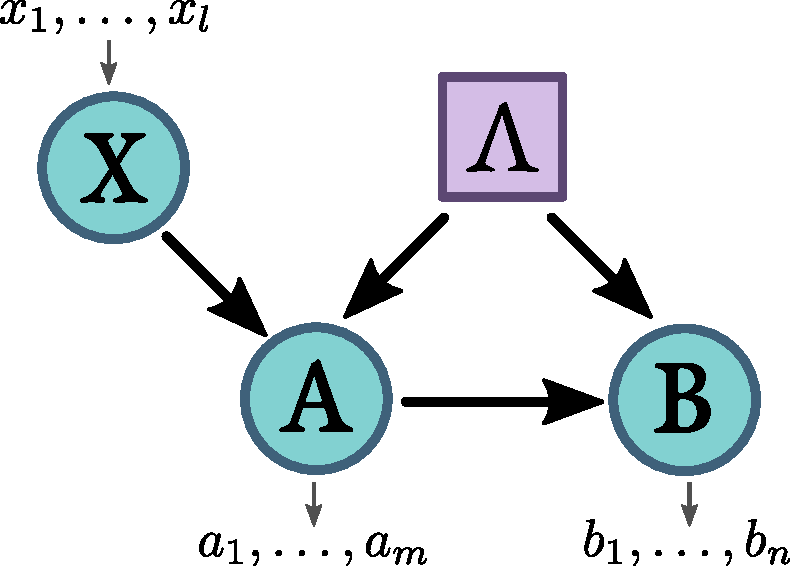
\includegraphics[width=.7\columnwidth]{images/instdag.pdf}
        \caption{\textcolor{blue}{ma se levamo quelle cose che stanno per dire input e ooutput nelle immagine? tipo lasiare la struttura pulita, magari il resto possiamo dirlo nella caption?} The DAG representing a general Instrumental scenario.}
        \label{fig:instdag}
    }

    \bigskip
    \parbox{.9\columnwidth}{
        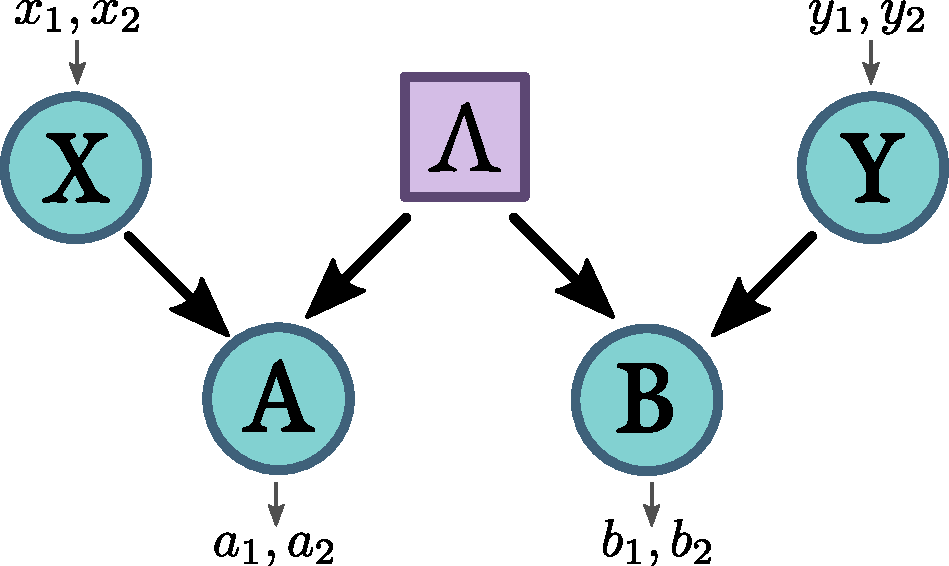
\includegraphics[width=.8\columnwidth]{images/chshdag.pdf}
        \caption{\textcolor{blue}{Davide non è piu conveniente mettere le 2 dags come 1 figura con a e b?} The DAG representing the CHSH scenario.}
        \label{fig:chshdag}
    }
\end{figure}

\section*{Instrumental causal structure}


\textcolor{blue}{Gonz proposta: Among all the possible causal structures, a particular interest has been devoted to the \textit{Instrumental causal structure} (see Fig.\ref{fig:instdag}) introduced by Pearl[] in the 90's with applications ranging from econometrics[] to clinical trial[]. One of the most important properties of instrumental variables is the fact that allow us to bound causal relations between variables solely from observational data. Like in the Bell tests where the inequalities allow us to test local-realism for a particular distribution, instrumental inequalities test whether we have a valid instrument.}\\
\textcolor{blue}{Recently has been experimentally proved that instrumental inequalities are also violated when considering quantum resources \cite{chaves2018}, thus opening several venues for future research such as device-independent cryptography [], random number generation[] and basically any application that until now has been linked with the Bell scenario.}\\

\textcolor{blue}{In light of the importance regarding the instrumental causal structure, we are interested in ...from the contextual point of view in order to better address the question of whether a ....could be possible.
Let us consider the instrumental structure depicted in Fig.\ref{fig:instdag} where X corresponds to the instrument, A and B the variables for which we are interested to bound the causal relation and $\lambda$ our quantum resource. If we allow the classical variables X, A, B to take the values $l,m,n$ respectively the Bayesian probability distribution for the i(j)-esimo outcome of A(B) given $x_k$ reads $P(a_i,b_j|x_k)$. From a classical perspective (and under some considerations even quantum) the upper-bound for the probability distribution}


The Instrumental causal structure is a widely studied
structure both for its simplicity and commonness.
It can be described by four random variables $\Lambda, X, A, B$ where $X$ and
$\Lambda$ are independent from the others while $B$ depends on $X$ only via the node $A$,
as graphically depicted in Fig.~\ref{fig:instdag}.

The consequences of these causal relations on the distributions of the four
variables have been throughly studied in previous works \cite{pearl1995,
bonet2001}.
Suppose that $X, A, B$ take $l,m,n$ different values and 
call $P(a_i b_j | x_k)$ the probability that $A$ and $B$ take, respectively, values $a_i$
and $b_j$, given that $X$ reads $x_k$.
Such system respects the following inequalities,
named \emph{Pearl's inequalities} \cite{pearl1995}:
\begin{equation} 
    \sum_{j=0}^{n} P(a_i b_j|x_{k(i,j)}) \le 1
    \label{eq:pearl_ineq}
\end{equation}
for all $i \in {1,\ldots, m}$ and for all the possible functions $k(i,j)$.

In \cite{bonet2001} Bonet showed that the polytope of allowed
correlation is not tightly bounded by \emph{Pearl's inequalities}.
For instance for $(l,m,n) = (3,2,2)$ the following inequality must also be satisfied:
\begin{multline}
    P(a_1 b_1 | x_1) + P(a_2 b_2 | x_1) + 
    P(a_1 b_1 | x_2) +\\+ P(a_2 b_1 | x_2) + 
    P(a_1 b_2 | x_3) \le 2
    \label{eq:bonet_ineq}
\end{multline}
along with other similar inequalities obtained by permuting the labels of
$a_i,b_j$ and $x_k$.


These inequalities are related to the one introduced in \cite{chaves2018}:
\begin{equation}
    -\avg{B}_{x_1} + 2 \avg{B}_{x_2} + \avg{A}_{x_1} - \avg{AB}_{x_1} +
    2\avg{AB}_{x_3} \le 3  
    \label{eq:rafael_ineq}
\end{equation}
which was experimentally violated in the same work, with a value of $3.790 \pm 0.013$.
As one can expect, with the same data it is also possible to violate inequality
\eqref{eq:bonet_ineq} with a value of $2.159 \pm 0.005$.

\section*{Exclusivity graph method}

The exclusivity graph method was primarily developed to study
non-contextual inequalities and obtain their quantum violation % cite something on NCI 
\cite{cabello2014} as well as for non-locality scenarios. %cite acin
In this formalism every possible event, i.e. every possible set of outcomes
$a_1^,\ldots, a_n$ of measurements $A_1,\ldots,A_n$ given settings
$x_1,\ldots,x_n$, is associated to a vertex in a (undirected) graph $G = (V, E)$.  
Two vertices $u, v \in V$ are then connected by an edge $uv \in E$ if and only
if they are exclusive, i.e.  if exists a measurement that can distinguish
between them. % In this case we write $u --- v$, else $u --/-- v$.

A linear constraint can be expressed as a linear function 
\begin{equation}
    I_w(p) = \sum_{\substack{a_1,\ldots,a_n\\x_1,\ldots,x_n}}
w_{\substack{a_1,\ldots,a_n\\x_1,\ldots,x_n}} p(a_1,\ldots,a_n|x_1,\ldots,x_n)
\end{equation}
 on the probabilities for each possible event.
In this framework this can be represented by weighted exclusivity graph $G$, and it
is possible to relate classical bound and quantum violation to well-known graph
invariants: the independence number $\alpha(G, w)$ and the Lovász theta
$\theta(G, w)$.

Here we briefly introduce these concepts and their relationships, a more
extensive and general treatment can be found in \cite{cabello2014, rabelo2014} %cite e acin

Consider a graph $G(V,E)$ with vertex weights $w$, and $|V| = n$ .
We call a \emph{characteristic labelling} for $U \subseteq V$ a vector $x_v \in
\{0,1\}^n$ such that $x_v = 1$ if $v \in U$ and $x_v = 0$ otherwise.

An \emph{independent set} or \emph{stable set} is a set
$S \subset V$ such that $uv \notin E$ for all $u,v \in S$.
The independence number $\alpha(G, w)$ is defined as the maximum number of
vertices (weighted with $w$) of an independent set of $G$.
Is also costumary to define the set $\STAB(G)$ as the convex hull of all the
characteristic labellings of stable sets:
\begin{equation}
    \STAB(G) = \{x : x \quad \text{is a stable labelling of}\quad G \}
    \label{eq:stab}
\end{equation}
using this definition the independence number becomes:
\begin{equation}
    \alpha(G,w) = \max\{w\cdot x: x \in \STAB(G)\}
    \label{eq:alphastab}
\end{equation}
From this definitions we can see that $\alpha(G,w)$ corresponds to the classical
bound of inequality, since it is exaclty the maximum over the convex set defined
by all the deterministic strategies respecting the exclusivity constraints.

We now call an \emph{orthonormal labelling} of dimension $d$ a map
$a_v:V\rightarrow\Real^d$ such that $a_v \cdot a_u = 0$ for all $uv \in E$ and
$|a_v|^2 = 1$, and we define the set $\TH(G)$ as:
\begin{multline}
    \TH(G) = \{x: x_v = a_v^1 \, \text{where $a_v$ is an} \\ \text{orthonormal labelling of $G$}\}
    \label{eq:thbody}
\end{multline}
It can be proved that this set includes all the possible quantum strategies, but
in general is larger as it contains also the ``almost quantum correlations''
described in .%cite acin almostq
\footnote{As proved in \cite{} this set corresponds to the step $1+AB$ of the
NPA hierarchy \cite{}.} %cite
Maximizing over $\TH(G)$ gives the Lovász theta:
\begin{equation}
    \theta(G,w) = \{w\cdot x : x \in \TH(G)\}
    \label{eq:lovasztheta}
\end{equation}
which upper-bounds the maximum quantum value.

Moreover this approach gives a useful condition to check if a given graph $G$
admits a quantum violation.
Indeed it can be proved that $\TH(G) = \STAB(G)$ if and only if $G$ does not
contain a cycle $C_n$ with $n \ge 5$ and odd, or its complement as an induced subgraph.
This follows directly from the so called ``sandwich theorem'' and the ``strong
perfect graph theorem'' \cite{knuth}.

\subsection{Exclusivity graph method applied to causal models}
The techniques presented in the previous section can be also employed to analyze
a certain class of causal models.
Suppose we have a causal scenario as in fig~\ref{fig:onelambda}, with
$k$ observable variables, $l$ instruments with no incoming edges, and a single
unobservable latent variable $\Lambda$.

\begin{figure}[h]
    \centering
    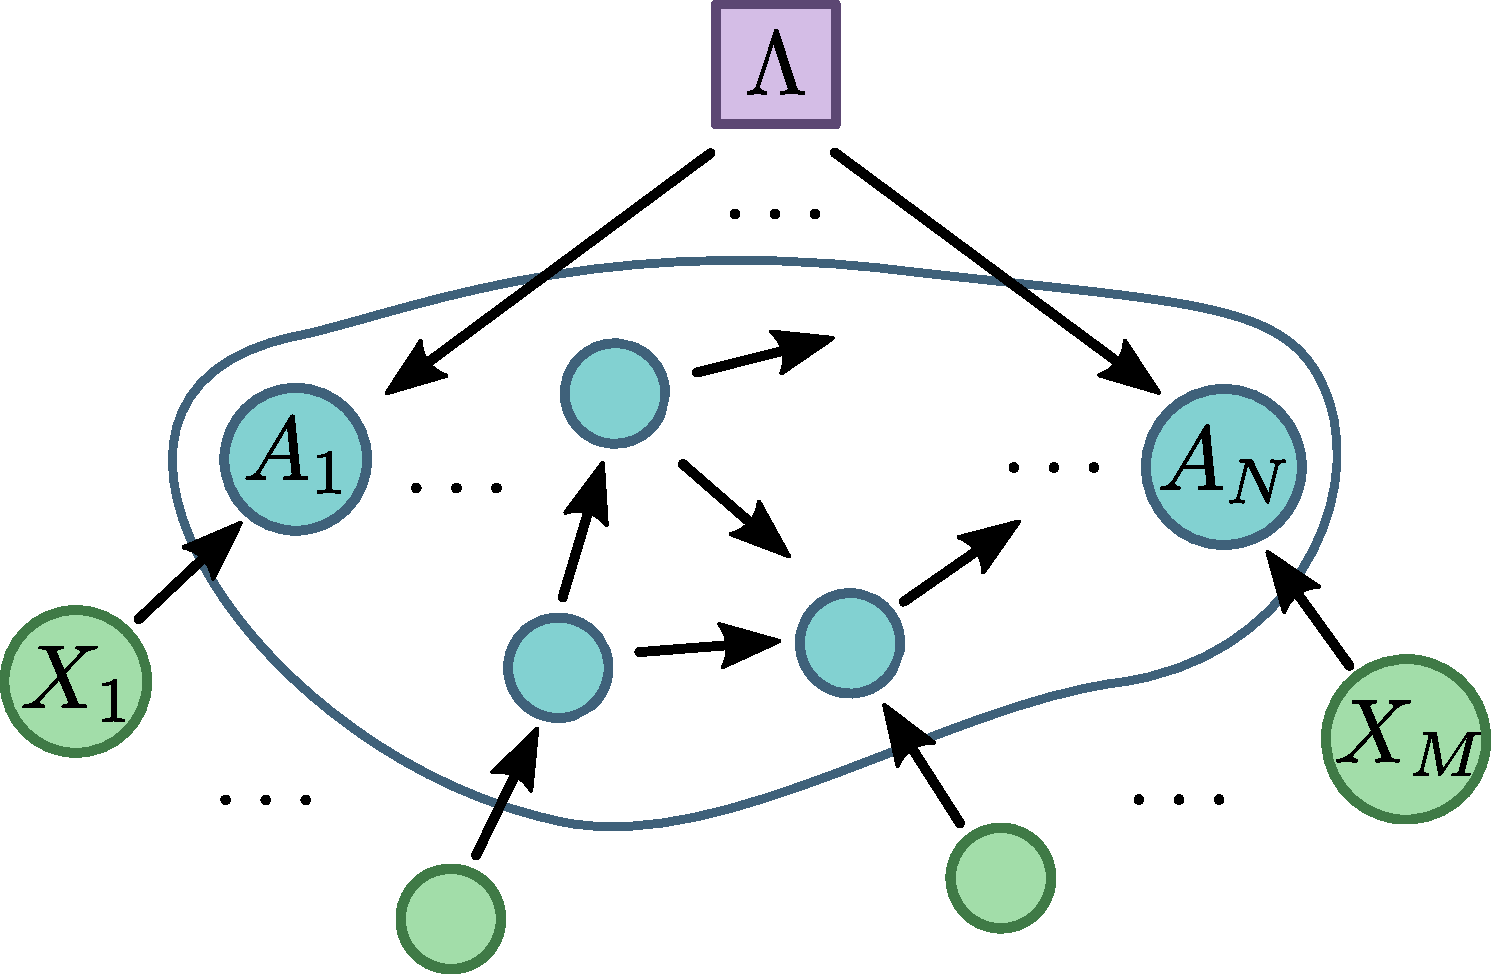
\includegraphics[width=.9\columnwidth]{images/onelambda.pdf}
    \caption{A general causal graph with $l$ instrument and a single latent
    variable.}
    \label{fig:onelambda}
\end{figure}

In this case we can associate with such a DAG a \emph{non-exclusivity} graph H
%(also called a \emph{confusability} graph) 
as follows:
\begin{itemize}
    \item Nodes are associated to events like $a | x$, where $a = (a_1,\ldots,a_k)$ and  $x = (x_1,\ldots,x_l)$.
    \item Two nodes $a | x$, and $a' | x'$ are linked by an edge if and only if 
        \begin{enumerate}
            \item for all $i,j \in \{1,\ldots,k\}$ if $A_i\,
                \rightarrow\, A_j$ then $\exists g_{ij} : g_{ij}(a_i) = a_j
                \et g_{ij}(a'_i) = a'_j$.
            \item for all $i\in \{1,\ldots,l\}$ and $j\in \{1,\ldots,k\}$ if
                $X_i\,\rightarrow\,A_j$ then $\exists f_{ij} : f_{ij}(x_i) = a_j
                \et f_{ij}(x'_i) = a'_j$.
        \end{enumerate}
\end{itemize}

To the complement of this graph, $G=\bar{H}$, and its subgraphs, the previous
methods can be applied to obtain inequalities with their respective quantum and
classical bounds.

\subsection{The Instrumental exclusivity graph}
\begin{figure*}[t]
    \centering
    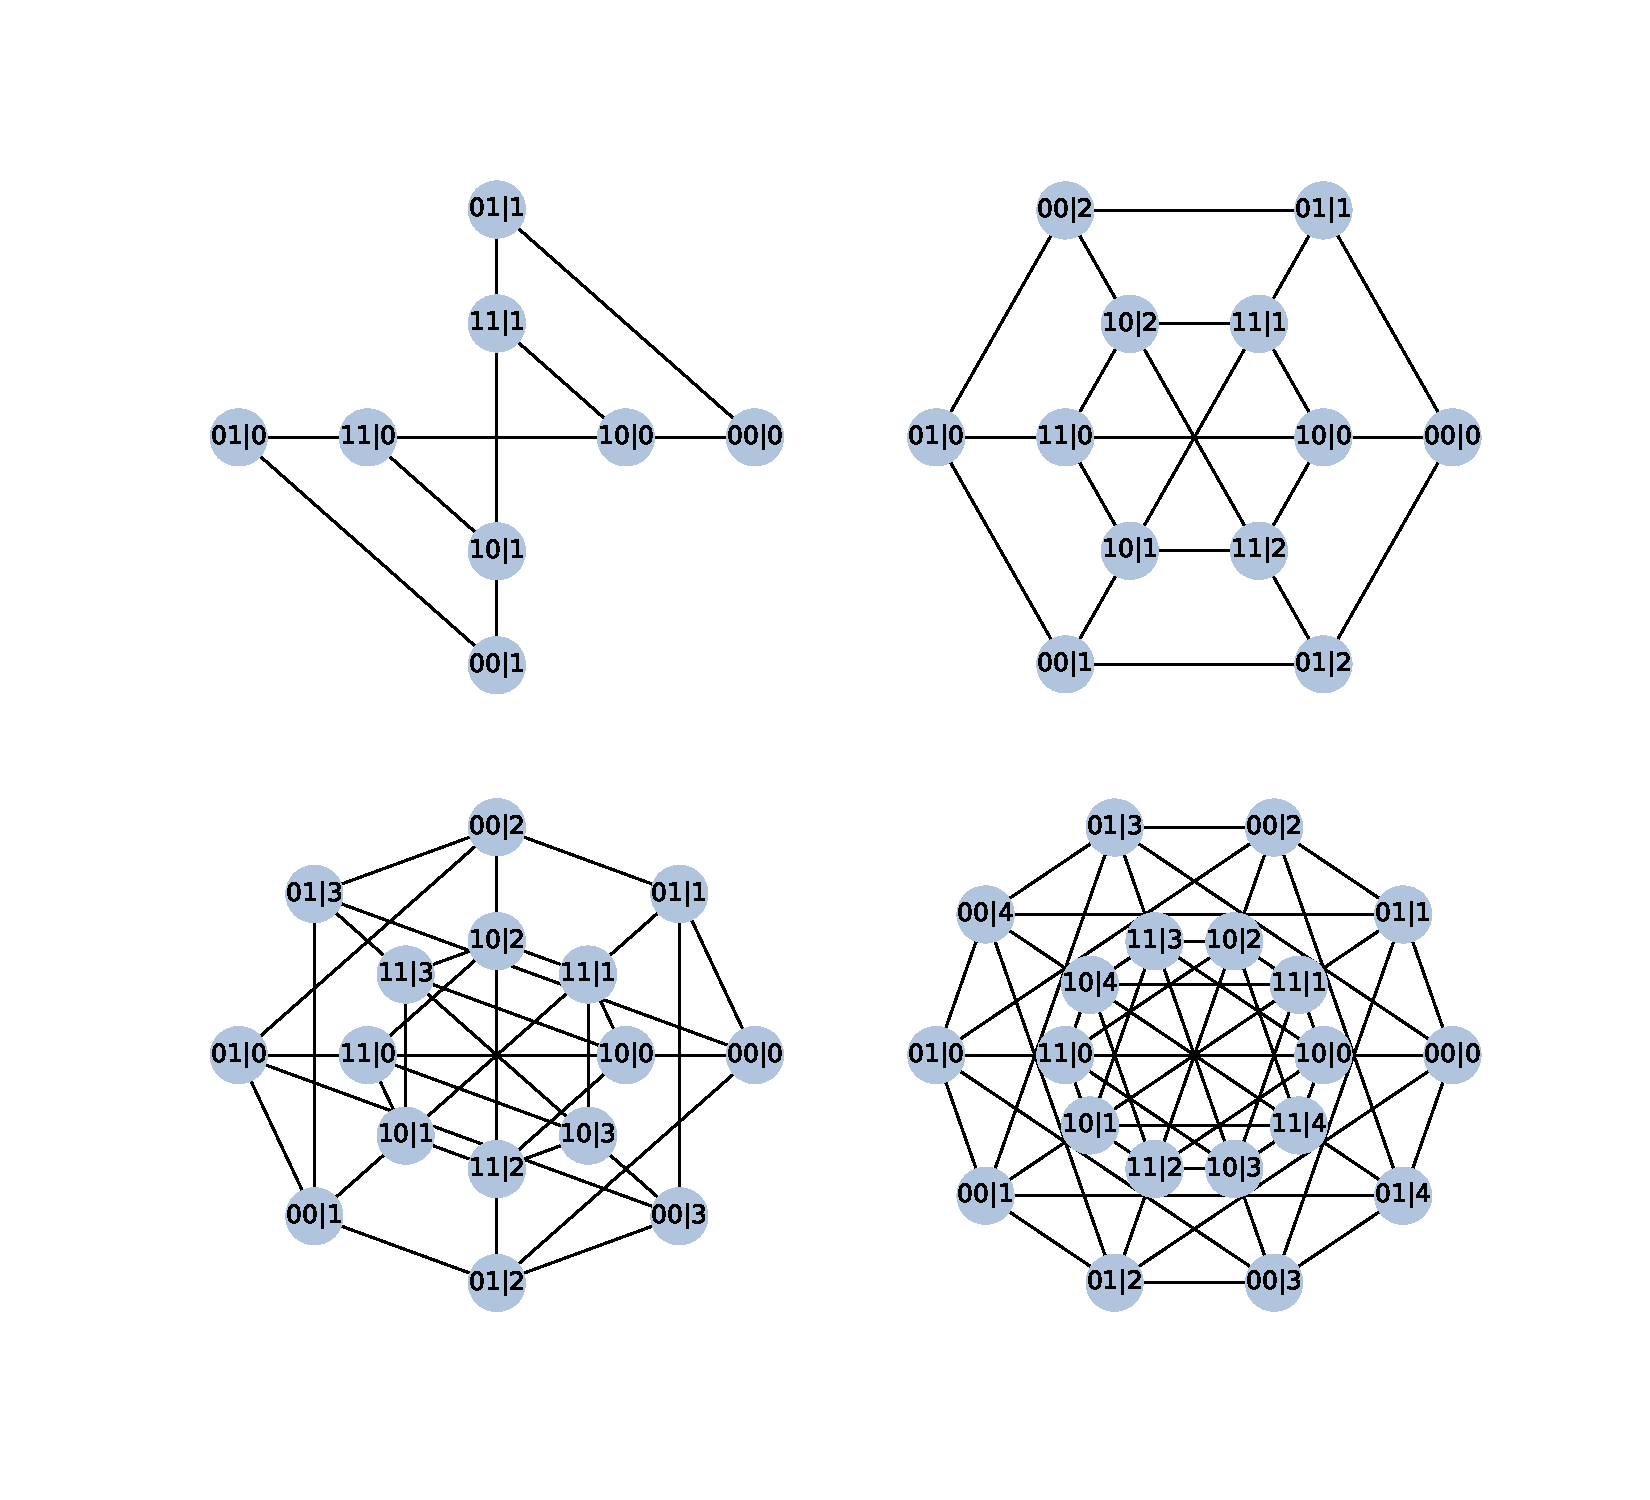
\includegraphics[width=.7\textwidth]{images/instrumental_exgraph.pdf}
    \caption{The exclusivity graph for the instrumental scenario for $l=2,3,4,5$
    from top left to bottom right. In the figure the bold lines represent
    cliques.}
    \label{fig:instrumental_exgraphs}
\end{figure*}

Many known results about the instrumental scenario, including the inequality
\eqref{eq:bonet_ineq}, can also be obtained using this formalism.  Restricting
for the moment to the case of of dichotomic observables ($n = m = 2$), we label
as $p(ab|x)$ with $a, b \in \mathcal{A} = \mathcal{B} = \{0,1\}$ and $x \in
\mathcal{X} = \{0,\ldots,l\}$, the probability of having outcomes $a$ and $b$
with setting $x$. 
As explained in the previous section we obtain the non-exclusivity graph for the
instrumental scenario by linking two events $ab|x$ and $a'b'|x'$ if exist two
functions $f:\mathcal{X} \rightarrow \mathcal{A}$ and $g:\mathcal{A} \rightarrow
\mathcal{B}$ such that:
\begin{align}
    a = f(x) \quad\text{and}\quad a'=f(x')\\
    b = g(a) \quad\text{and}\quad b'=g(a')
    \label{eq:non_exclusivity_condition}
\end{align}
Using this method we can construct the graph for various $l$, as shown in figure
\ref{fig:instrumental_exgraphs}, and use the methods described earlier to obtain
classical and quantum bounds for several inequalities in the instrumental
scenario. 

First, we immediately obtain the result that there is no quantum violation in
the case of $l=2$, since the corresponding exclusivity graph (and its
complement) does not contain any odd cyclic graph with more than $5$ vertices.  

\begin{figure}[h]
    \centering
    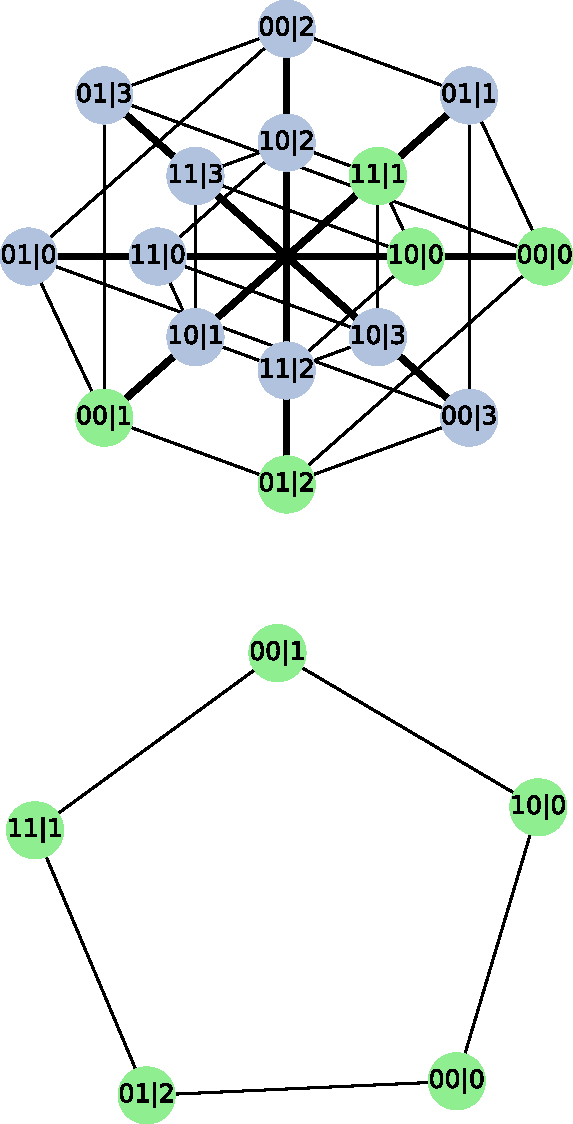
\includegraphics[width=.8\columnwidth]{images/instrumental_c5.pdf}
    \caption{The exclusivity graph of the bonet inequality.}
    \label{fig:bonetexc}
\end{figure}

For $l\ge3$ instead we see that there is a violation for the inequality \eqref{eq:bonet_ineq},
since it forms a $C_5$ cyclic graph, i.e. the pentagon depicted in
fig.~\ref{fig:bonetexc}.
Knowing that $\alpha(C_n) = \lfloor n/2 \rfloor$ we immediately derive that the classical limit is $2$.
Analogously knowing that $\theta(C_n) = n\cos(\pi/n)/(1+\cos(\pi/n))$ we get
$\sqrt{5}$ as an upper bound for the quantum limit.

In this framework \eqref{eq:bonet_ineq} seems analogous to the KCBS contextual
inequality. %cite
The difference here is that the quantum limit is not $\sqrt{5}$, which we cannot
obtain in a bipartite scenario.
To find a tight bound we must apply other methods to our graph, like the ones in
\cite{rabelo2014}, using which we find a value of $(3+\sqrt{2})/2$.

It can be easily proved (see Methods) that no other odd anticycle beside
$C_5$ is present for any $l$, so from this point of view, we can say that any
quantum violation for a general $l22$ instrumental scenario has essentially the
same origin: it stems from the non classicality of the $C_5$ graph.

This does not mean that different inequalities cannot be devised by clever
choices of vertices and weights.
For example the inequality for the $422$ scenario presented in
\cite{rand_internal_report}
\begin{equation}
    \avg{AB}_1 -  \avg{AB}_2 + \avg{B}_0 - \avg{B}_3 \le 2
    \label{eq:422_ineq}
\end{equation}
correponds to the two sets of events whose
exclusivity graphs are depicted in fig.~\ref{fig:422_exgraph}.
The maximum classical value for both, given by the independence number of the
graphs, is $3$, while their minimum is $1$, which gives the maximum value of $2$
as in \eqref{eq:422_ineq} when taken with opposite sign.
This inequality has a structure very similar to the CHSH (showed in
fig.\ref{fig:chsh_exgraph}), and, as pointed out above, both arise from the
non-classicality of the $C_5$ graph.

\begin{figure}[b]
    \centering
    \parbox{.9\columnwidth}{
        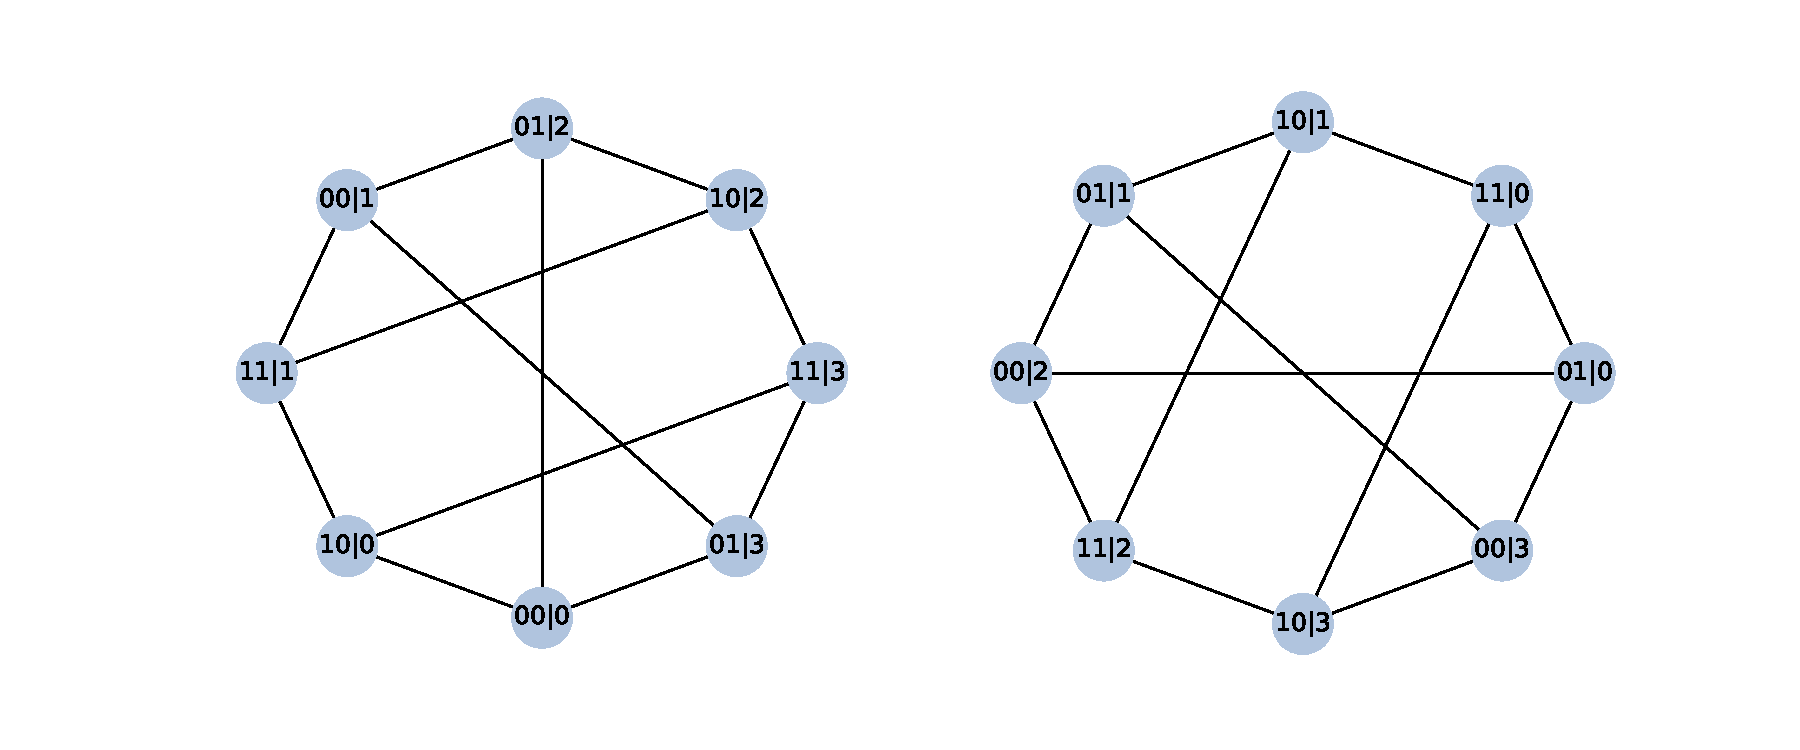
\includegraphics[width=\columnwidth]{images/422_exgraph.pdf}
        \caption{The exclusivity graph for the $422$ Instrumental scenario.}
        \label{fig:422_exgraph}
    }

    \bigskip
    \parbox{.9\columnwidth}{
        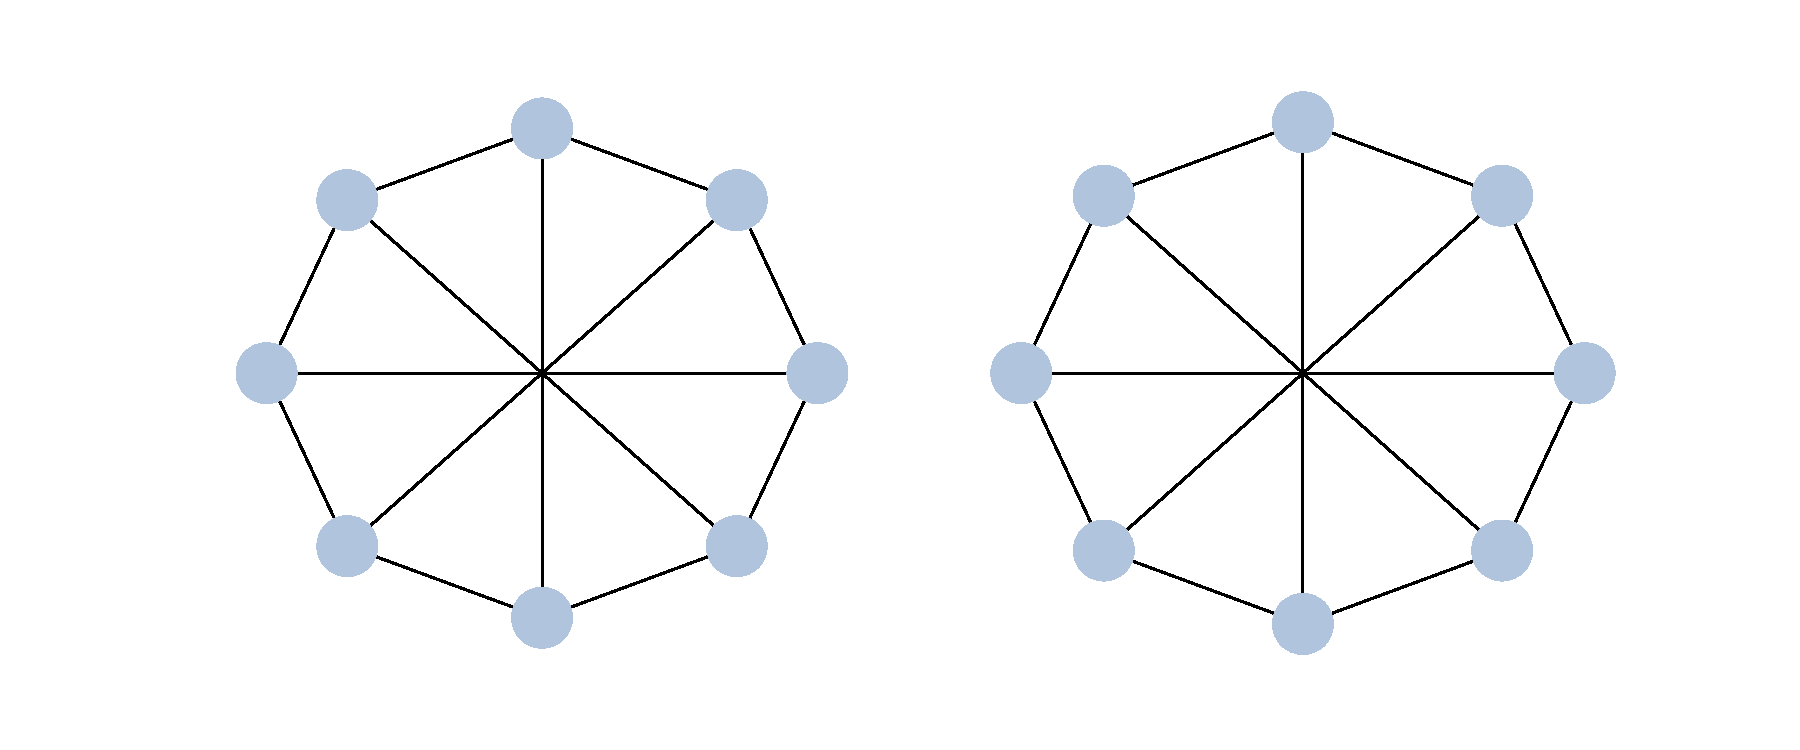
\includegraphics[width=.8\columnwidth]{images/chsh_exgraph.pdf}
        \caption{The exclusivity graphs for the the CHSH scenario.}
        \label{fig:chsh_exgraph}
    }
\end{figure}

\subsection{Finding optimal inequalities}
The presence of an odd cycle graph guarantees only that $\STAB(G) \subset
\TH(G)$, but does not say anything on the values of $\theta(G)$ and $\alpha(G)$.
Nonetheless, if that condition is satisfied there must be some optimal choice of
weights $w$ for which we can obtain a maximum quantum violation.
Formally if $n$ is the number of nodes of $G$, we want to find the maximum:
\begin{equation}
    \max_{w \in [0,1]^n} \{\theta(G,w) - \alpha(G,w)\}
    \label{eq:maxonw}
\end{equation}

Using the definition \eqref{eq:lovasztheta} and \eqref{eq:alphastab}, and
remembering that $\STAB(G)$ is a convex hull of a finite number of
characteristic labellings we can rewirte the previous maximization as:
\begin{align}
    \Delta &= \min \{I_y : y \, \text{is a maximal stable labelling}\}
    \label{eq:maximize_w_delta}\\
    I_y &= \max_{\substack{w \in [0,1]^n\\x \in \TH(G)}} \{w\cdot (x - y)\}
    \label{eq:maximize_w_I}
\end{align}

The maximization \eqref{eq:maximize_w_I} for each $y$ is efficient, being a
semi-definite program, but unfortunately it has to be run for each maximal
stable set in $G$ which are $\sim 3^{n/3}$ in the worst case.
Also to enumerate all the maximal independent sets we used the Tomita version of
the Bron–Kerbosch algorithm which has the same worst case complexity. % cite

\section{Methods}
\subsection{There are no cycles $C_n$ with $n \ge 7$ in the $d22$ instrumental scenario.}
\label{sec:c5only_proof}
Here we prove that there cannot be a odd antihole with more than $5$ vertices in
the exclusivity graph associated to an instrumental scenario of the type $d22$.

\begin{figure}[h]
    \centering
    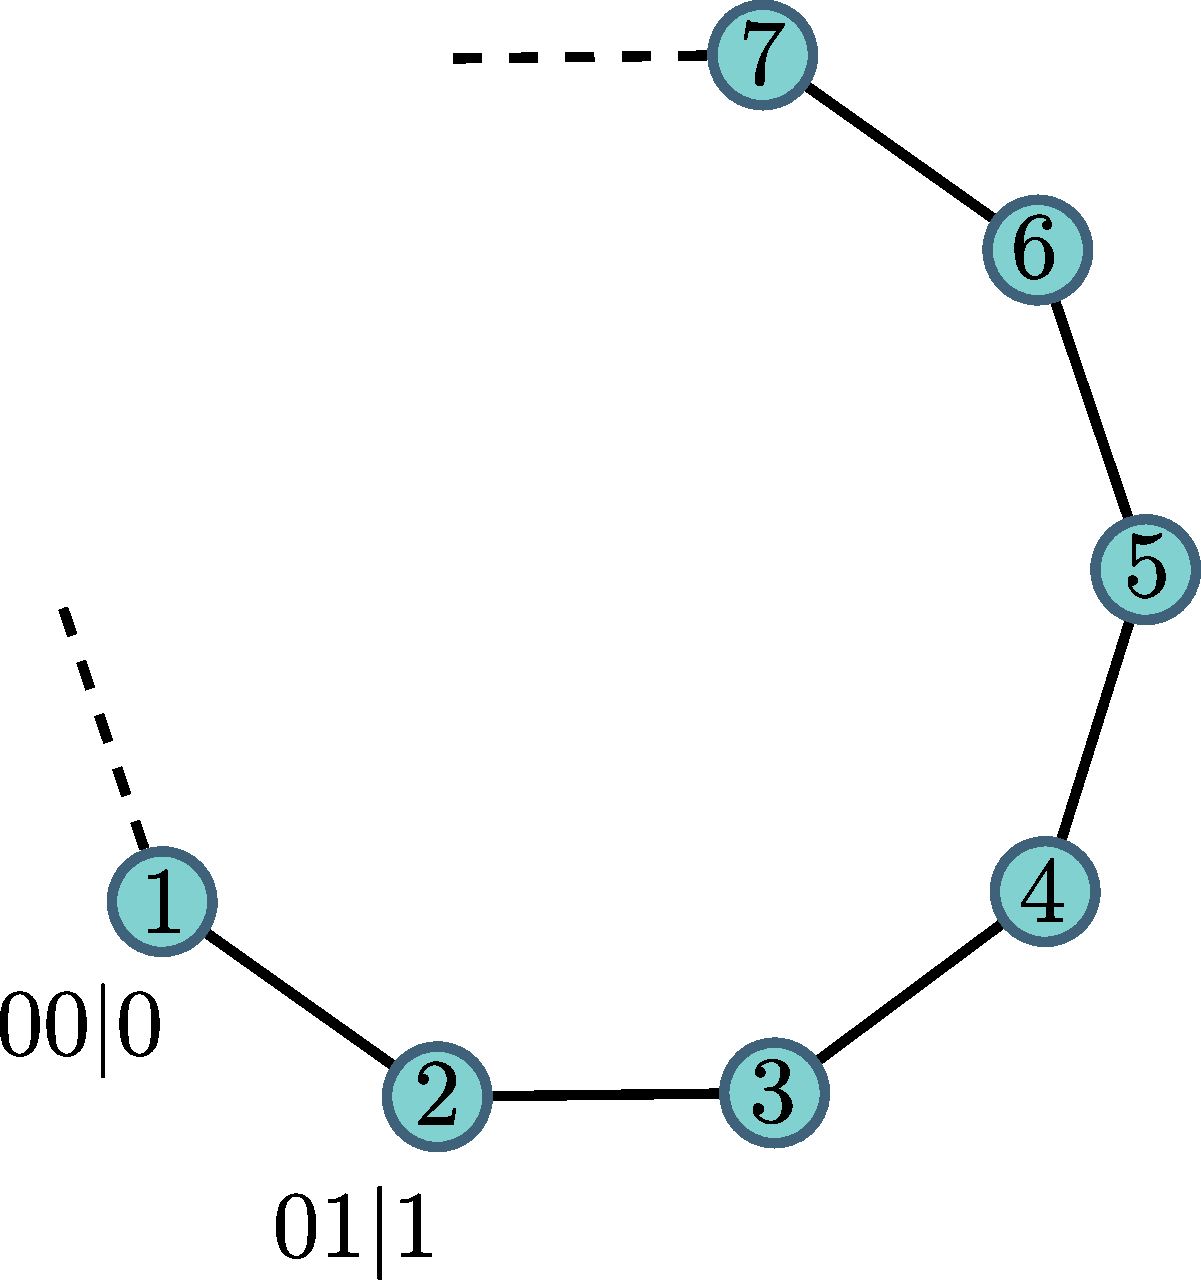
\includegraphics[width=.6\columnwidth]{images/cycle_proof.pdf}
    \caption{Proof of the impossibility of having cycles with $7$ nodes or more
    in the $d22$ scenario.}
    \label{fig:cycle_graph_proof}
\end{figure}
Remind that, from the exclusivity conditions \eqref{eq:non-exclsivity_conditions},
given two events $ab|x$ and $a'b'|x'$, they are connected by edge if one of
these two conditions is true:
\begin{enumerate}
    \item $x=x'$.\label{en:rule1}
    \item $a=a'$ and $b \neq b'$.\label{en:rule2}
\end{enumerate}
Suppose we have a cycle $C_n$ with $n \ge 7$, as in fig.~\ref{fig:cycle_graph_proof},
and consider node $2$ which correspond to an event which we can arbitrarily identify
with $00|0$.
Among its neighbors $1$ and $3$, one will necessarily need to satisfy rule 
\ref{en:rule2} (they cannot both satisfy rule \ref{en:rule1} or 
the three nodes would be a clique).
So without loss of generality we can assign the event $01|1$ to $3$.
Since nodes $5,6,7$ must not satisfy rule \ref{en:rule2} with both $2$ and $3$ 
they must have $a = 1$.
Moreover $7$ and $5$ must have the same $b$, different from $6$.
In the same way $1$ must not satisfy rule \ref{en:rule2} with $6,5$ and $3$, so it
needs to have $a=0$ and $b=1$.
But now, since we only have values $\{0,1\}$ for $a$, we cannot avoid $4$ 
to be linked to one of the nodes $1,2,6,7$.

\begin{thebibliography}{}
    \bibitem{pearl1995} J.Pearl, {\em On the testability of causal models with
        latent and instrumental variables}, 
        Proceedings of the Eleventh conference on Uncertainty in artificial
        intelligence. Morgan Kaufmann Publishers Inc. (1995).
    \bibitem{bonet2001} B.Bonet, {\em Instrumentality tests revisited},
        Proceedings of the Seventeenth conference on Uncertainty in artificial
        intelligence. Morgan Kaufmann Publishers Inc. (2001).
    \bibitem{chaves2018} R.Chaves, G.Carvacho, I.Agresti, V.Di Giulio, L.Aolita,
        S.Giacomini, F.Sciarrino, 
        {\em Quantum violation of an instrumental test}, 
        Nature Physics 14.3 291 (2018).
     \bibitem{himbeeck2018} T.Van Himbeeck, J.B. Brask, S.Pironio, R.Ramanathan, A.B.Sainz, E. Wolfe, 
        {\em Quantum violations in the Instrumental scenario and their relations to the Bell scenario},
        arXiv preprint arXiv:1804.04119 (2018).
         (2014).
     \bibitem{cabello2014} A.Cabello, S.Severini, A.Winter,
         {\em Graph-theoretic approach to quantum correlations}, 
         Physical review letters, 112(4), 040401 (2014).
     \bibitem{rabelo2014} Rabelo, R., Duarte, C., López-Tarrida, A. J., Cunha, M. T., Cabello, A. (2014). {\em Multigraph approach to quantum non-locality.} Journal of Physics A: Mathematical and Theoretical, 47(42), 424021.
     \bibitem{kcbs2008} Klyachko, A. A., Can, M. A., Binicioğlu, S., Shumovsky, A. S. (2008). {\em Simple test for hidden variables in spin-1 systems.} Physical review letters, 101(2), 020403.
     
%\bibitem{} , {\em },  ().
\end{thebibliography}

\end{document}
